%% =====================================================================
\section{Experiments}
\label{sec:experiments}

\paragraph{Setup.}
All runs used CPUs except the GPU training runs named in the text. \FiveB, \FiveA and \Mfour ran on a 2-core machine with one
thread per process; Methods 1--3, \FiveC, \Msix, \Mseven and the external baselines on a 4-core, 15\,GB machine, often several
jobs at once, so times are comparable within a table only. Every method sees the same instances (\S\ref{sec:data}), and every
number below is generated by script from the harness's result files. Means are over solved instances; a superscript gives the
solved fraction (random states) or the number of puzzles run (Santa) when it is below the full count.

We organise the results in three comparisons, as the paper's claims are of three kinds: \emph{reproductions against their
originals} (\S\ref{sec:exp-repro}), \emph{our methods against baselines and reproductions} on random states
(\S\ref{sec:exp-ours}), and \emph{our methods against published numbers} on Santa 2023 (\S\ref{sec:exp-published}); then we
ask how far everything is from optimal (\S\ref{sec:exp-bound}).

%% ---------------------------------------------------------------------
\subsection{Reproductions against their originals}
\label{sec:exp-repro}

\paragraph{\Mone and exact optima.}
Breadth-first search from all four solved orientations visits all \StatesSquareThree{}, \StatesSquareFour{} and
\StatesSquareFive{} states of the \Sq{3}, \Sq{4} and \Sq{5}; their diameters are \GodSquareThree{}, \GodSquareFour{} and
\GodSquareFive{} moves. The \Sq{3} (the ``Floppy Cube'') values agree with the published ones for the same move set; for the
\Sq{4} and \Sq{5} we found no published value. IDA* solves random Squares optimally as follows: \MoneSquareCoverage{} (120\,s per
state; \MoneSquareFiveTime\,s per \Sq{5} on average). At $N=6$ the max-cluster heuristic is too weak and every search ran out of
time. On the \Cu{3}, the pattern databases have exactly the sizes of Korf's~\cite{korf1997optimal}; on 100 random scrambles of
12 moves IDA* returned an optimal solution for \MoneDTwelveSolved{} within 120\,s each (\MoneDTwelveHTM{} HTM on average, optima
between \MoneDTwelveMin{} and \MoneDTwelveMax{}). On \MoneRandTried{} random states it found no solution within \MoneRandMin{}
minutes each, after about $\MoneRandNodes\cdot10^{10}$ nodes, proving only that the optimum exceeds \MoneRandBound{} moves. Korf
reported optimal random \Cu{3} solutions with days of CPU time per state in 1997; our reproduction is correct but not fast enough
for that benchmark on four cores.

\begin{table}[t]
\caption{Optimality on the smallest Squares. ``Gap'' = mean HTM above the exact optimum over solved instances; ``optimal'' =
instances solved in exactly the optimal length. \FiveA was evaluated for $N\ge4$ only.}
\label{tab:optimal}
\small\setlength{\tabcolsep}{4pt}
\begin{tabular}{@{}lrrlrrr@{}}
\toprule
Puzzle & God's & mean opt. & Method & solved & gap & optimal \\
\midrule
\multirow{4}{*}{3$\times$3} & \multirow{4}{*}{6} & \multirow{4}{*}{3.6} & \Mfour ($W{=}4096$) & 10/10 & 0.0 & 10/10 \\
 & &  & \FiveA & -- & -- & -- \\
 & &  & \FiveB & 10/10 & 1.2 & 1/10 \\
 & &  & \Mtwo, \Mthree, \FiveC & 10/10 & 0.6 & 5/10 \\
\midrule
\multirow{4}{*}{4$\times$4} & \multirow{4}{*}{10} & \multirow{4}{*}{6.4} & \Mfour ($W{=}4096$) & 10/10 & 0.0 & 10/10 \\
 & &  & \FiveA & 10/10 & 0.0 & 10/10 \\
 & &  & \FiveB & 10/10 & 7.0 & 0/10 \\
 & &  & \Mtwo, \Mthree, \FiveC & 10/10 & 4.0 & 3/10 \\
\bottomrule

\end{tabular}
\end{table}

\paragraph{\Mfour against CayleyPy.}
On the Square, our per-size networks behave as CayleyPy reports for cubes: they found the optimum on every \Sq{3} and \Sq{4}
instance (\OptMfourThree{} and \OptMfourFour{}, Table~\ref{tab:optimal}), matched \Mone's optimal mean on the \Sq{5}, and wider
beams help (Figure~\ref{fig:m4width}): on the \Sq{8}, \Mfour solved \MfourEightSolvedWSixteen{} states at $W{=}16$,
\MfourEightSolvedWTwoFiftySix{} at $W{=}256$ and all from $W{=}1024$ on, at \MfourEightTimeWFourK\,s per state for $W{=}4096$. On the
\Cu{3}, with 250$\times$ less training data than the original, our model solved short scrambles but none of 10 random states at
$W\in\{256, 1024, 4096\}$ and none of 4 at $W=16{,}384$: we did not reproduce CayleyPy's \Cu{3} result, which is a statement about
our compute, not about the method.

\begin{figure}[t]
\centering
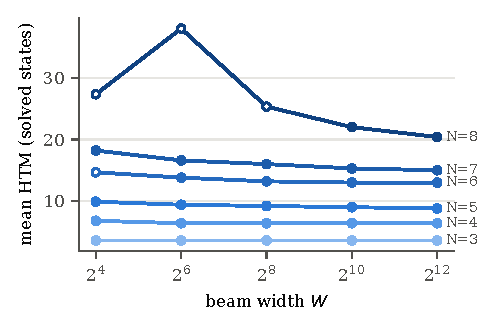
\includegraphics[width=\columnwidth]{figures/m4_width.pdf}
\caption{\Mfour: mean solution length against beam width $W$, one per-size network for each Square size $N=3,\dots,8$ (10 states
each; means over solved states). Hollow markers: not all 10 states solved.}
\label{fig:m4width}
\end{figure}

\paragraph{\Mfour with GPU-trained models.}
\label{sec:m4gpu}
A second set of Square models, trained on a Colab T4 with the ``large'' preset (1.27M parameters and 256M examples at $N=8$,
about 7 minutes per model), gives the same lengths as the CPU-trained models up to $N=6$ and is better only at $N=8$
(\MfourGpuEightGpu{} against \MfourGpuEightCpu{} HTM, shorter on \MfourGpuEightShorter{} of 20 states and longer on none;
Table~\ref{tab:m4gpu}). The larger model is the default at $N=8$ only.

\begin{table}[t]
\caption{\Mfour on the same 20 random Squares per size, same CPU, $W{=}4096$: committed CPU-trained models against the GPU-trained
``large'' models. Last column: states with a shorter / longer solution with the GPU model. Every state was solved by both.}
\label{tab:m4gpu}
\small
\begin{tabular}{@{}rrrrrr@{}}
\toprule
$N$ & $n$ & optimal & CPU-trained & GPU-trained & shorter / longer \\
\midrule
3 & 20 & 3.75 & 3.75 & 3.75 & 0 / 0 \\
4 & 20 & 6.70 & 6.70 & 6.70 & 0 / 0 \\
5 & 20 & -- & 9.10 & 9.10 & 0 / 0 \\
6 & 20 & -- & 12.60 & 12.60 & 0 / 0 \\
7 & 20 & -- & 15.40 & 15.60 & 0 / 4 \\
8 & 20 & -- & 20.30 & 18.80 & 12 / 0 \\
\bottomrule

\end{tabular}
\end{table}

\paragraph{\Msix and one run of KMCoders' program against KMCoders' published lengths.}
Table~\ref{tab:repro-kmc} compares the two ways of reproducing KMCoders on the Santa puzzles. Our reproduction from the write-up
(\Msix) is \MsixOverPubMin{}--\MsixOverPubMax{}$\times$ their published lengths at every size, but it is the best of our
non-KMCoders methods from $N=6$ on (Table~\ref{tab:santa}). One run of their own program is only 7--18\% longer than the published
lengths. The gap between \Msix and B2 is what the write-up leaves out (\S\ref{sec:m6}); the gap between B2 and B1 is what many runs
and tuning bought in the competition, and it is what \Mseven goes after.

\begin{table}[t]
\caption{Reproducing KMCoders on the Santa 2023 cubes (mean QTM). B1: their published solutions; B2: one run of their program
(puzzles run in brackets); \Msix: our reproduction from their write-up. Ratios to B1.}
\label{tab:repro-kmc}
\small\setlength{\tabcolsep}{4pt}
\begin{tabular}{@{}rrrrrr@{}}
\toprule
$N$ & B1 published & B2 one run & B2 / B1 & \Msix & \Msix / B1 \\
\midrule
4 & 66.7 & 77.0 (43) & 1.15 & 109.4 & 1.64 \\
5 & 97.1 & 114.2 (19) & 1.18 & 159.3 & 1.64 \\
6 & 161.0 & 179.3 (6) & 1.11 & 276.0 & 1.71 \\
7 & 208.8 & 232.8 (4) & 1.11 & 356.2 & 1.71 \\
8 & 291.3 & 310.7 (3) & 1.07 & 468.7 & 1.61 \\
9 & 354.7 & 390.0 (3) & 1.10 & 572.7 & 1.61 \\
\bottomrule

\end{tabular}
\end{table}

%% ---------------------------------------------------------------------
\subsection{Our methods against baselines and reproductions (random states)}
\label{sec:exp-ours}

\begin{table*}[t]
\caption{Rubik's Square, random states: mean HTM of every method on the same instances. ``optimal'': exact BFS ($N\le4$) or
\Mone's IDA* ($N=5$). \Mfour: per-size network, $W{=}4096$. Bold: shortest method that solved every instance of that size. A
superscript gives the solved fraction when below 100\%; ``--'' = not run (no model or out of scope), ``--$^{0/k}$'' = tried, none
solved. Methods 2, 3, 5B and 5C solved every instance.}
\label{tab:square}
\small
\begin{tabular}{@{}rrrrrrrrr@{}}
\toprule
$N$ & $n$ & optimal & \Mfour & \FiveA & \FiveB & \Mtwo & \Mthree & \FiveC \\
\midrule
3 & 10 & 3.6 & 3.6 & -- & 4.8\,$\pm$\,1.0 & 10/10 & 0.59 & 0.0 \\
4 & 10 & 6.4 & 6.4 & 6.4 & 13.4\,$\pm$\,1.8 & 10/10 & 1.16 & 0.0 \\
5 & 10 & -- & 8.8 & 10.0 & 22.2\,$\pm$\,2.3 & 10/10 & 1.43 & 0.2 \\
6 & 10 & -- & 13.0 & 15.0 & 28.0\,$\pm$\,2.5 & 10/10 & 1.39 & 0.1 \\
7 & 10 & -- & 15.0 & 23.5$^{4/10}$ & 41.8\,$\pm$\,4.4 & 10/10 & 1.66 & 0.2 \\
8 & 10 & -- & 20.4 & 56.4 & 61.6\,$\pm$\,5.4 & 10/10 & 2.00 & 0.6 \\
9 & 10 & -- & -- & 70.0 & 83.2\,$\pm$\,6.1 & 10/10 & 2.26 & 1.0 \\
10 & 10 & -- & -- & 85.5$^{8/10}$ & 103.4\,$\pm$\,6.1 & 10/10 & 2.38 & 1.6 \\
11 & 10 & -- & -- & -- & 121.4\,$\pm$\,7.5 & 10/10 & 2.41 & 3.3 \\
12 & 10 & -- & -- & --$^{0/1}$ & 143.0\,$\pm$\,6.4 & 10/10 & 2.47 & 5.9 \\
13 & 5 & -- & -- & -- & 170.4\,$\pm$\,7.3 & 5/5 & 2.59 & 7.0 \\
14 & 5 & -- & -- & -- & 221.2\,$\pm$\,17.6 & 5/5 & 2.98 & 11.9 \\
15 & 5 & -- & -- & -- & 242.8\,$\pm$\,20.9 & 5/5 & 2.92 & 13.0 \\
16 & 5 & -- & -- & -- & 280.0\,$\pm$\,15.8 & 5/5 & 3.03 & 15.8 \\
17 & 5 & -- & -- & -- & 298.4\,$\pm$\,30.8 & 5/5 & 2.93 & 21.1 \\
18 & 5 & -- & -- & -- & 354.8\,$\pm$\,11.5 & 5/5 & 3.17 & 34.0 \\
19 & 5 & -- & -- & -- & 394.4\,$\pm$\,23.5 & 5/5 & 3.22 & 43.0 \\
20 & 5 & -- & -- & -- & 486.4\,$\pm$\,43.3 & 5/5 & 3.64 & 60.3 \\
\bottomrule

\end{tabular}
\end{table*}

\begin{table*}[t]
\caption{Rubik's Cube, random states: mean HTM of every method on the same instances (bold: shortest), then \FiveC's QTM, its
length divided by $N^2/\ln N$ and its time per state on the 4-core machine. Every method solved every instance.}
\label{tab:cube}
\small
\begin{tabular}{@{}rrrrrrrrr@{}}
\toprule
$N$ & $n$ & \FiveB & \Mtwo & \Mthree & \FiveC & \FiveC QTM & \FiveC / $(N^2/\ln N)$ & \FiveC time (s) \\
\midrule
3 & 2 & 52.0 & \textbf{21.0} & \textbf{21.0} & \textbf{21.0} & 31.0 & 2.6 & 0 \\
4 & 2 & 246.0 & 219.0 & \textbf{192.5} & 196.0 & 224.5 & 17.0 & 1 \\
5 & 2 & 452.5 & 319.5 & 258.0 & \textbf{253.0} & 281.0 & 16.3 & 1 \\
6 & 2 & 724.5 & 574.5 & 464.5 & \textbf{437.0} & 481.5 & 21.7 & 4 \\
7 & 2 & 1,045.0 & 811.0 & 633.0 & \textbf{564.0} & 614.5 & 22.4 & 7 \\
8 & 2 & 1,510.5 & 1,131.0 & 897.5 & \textbf{806.5} & 863.0 & 26.2 & 17 \\
10 & 2 & 2,260.5 & 1,900.5 & 1,509.0 & \textbf{1,196.5} & 1,256.5 & 27.6 & 37 \\
15 & 1 & 5,280.0 & 4,565.0 & 3,578.0 & \textbf{2,765.0} & 2,927.0 & 33.3 & 223 \\
20 & 1 & 9,904.0 & 8,259.0 & 6,612.0 & \textbf{4,925.0} & 5,188.0 & 36.9 & 158 \\
\bottomrule

\end{tabular}
\end{table*}

\paragraph{Main comparison.}
Methods 2, 3 and \FiveC solved all Square instances (\SqSolvedFiveC{}) and all cube instances (\CuSolvedFiveC{}), and \FiveB
solved all \SqSolved{} of \SqTotal{} Squares and all \CuSolved{} of \CuTotal{} cubes (Tables~\ref{tab:square} and~\ref{tab:cube}).
Which method is shortest depends on the size. On the smallest Squares, exact search and \Mfour's per-size networks are optimal.
From the \Sq{9} on, where no per-size network exists, \FiveC is the shortest method: strictly shorter than \Mthree at
\SqFiveCBetter{} of the 12 sizes from 9 to 20 (\SqTwentyHTMFiveC{} against \SqTwentyHTMMthree{} and \SqTwentyHTMMtwo{} moves for
\Mthree and \Mtwo on the \Sq{20}). On the cube, \FiveC is the shortest method at every size from $N=5$ on. On the \Cu{20} it needs
\CuTwentyHTMFiveC{} moves against \CuTwentyHTMMthree{} for \Mthree, \CuTwentyHTMMtwo{} for \Mtwo and \CuTwentyHTM{} for \FiveB, in
\FiveCTwentyMin{} minutes. Batching alone (\Mthree against \Mtwo, which share every other stage) saves \MthreevsMtwoTwenty\% there;
\FiveC's schedule saves another \FiveCGainTwenty\% on top. \FiveB is the longest of the four at every cube size: it searches for each
stage's moves with learned and abstraction heuristics instead of applying prescribed 3-cycles, and pays for that generality in
length.

\paragraph{Statistics with 20 states per size.}
\label{sec:ci}
Table~\ref{tab:ci} repeats the cube comparison of Methods 2, 3 and \FiveC with 20 states per size and 95\% confidence intervals, and
gives the paired difference \FiveC$-$\Mthree on the same states. \FiveC is significantly shorter than \Mthree from $N=5$ on, and the
gap grows steadily with $N$; at $N=4$, with one center and one wing cluster and nothing to batch, the difference is not
significant.

\begin{table}[t]
\caption{Cube, 20 random states per size: mean HTM $\pm$ 95\% confidence half-width, and the paired difference \FiveC$-$\Mthree
on the same states ($^\ast$: interval excludes 0).}
\label{tab:ci}
\small\setlength{\tabcolsep}{2.5pt}
\begin{tabular}{@{}rllllr@{}}
\toprule
$N$ & \Mtwo & \Mthree & \FiveC & \FiveC$-$\Mthree & $n$ \\
\midrule
3 & 20.7 $\pm$ 0.4 & 20.7 $\pm$ 0.4 & 20.7 $\pm$ 0.4 & +0.0 $\pm$ 0.0 (+0.0\%) & 20 \\
4 & 212.6 $\pm$ 4.5 & 186.8 $\pm$ 5.0 & 184.1 $\pm$ 4.1 & -2.8 $\pm$ 3.4 (-1.5\%) & 20 \\
5 & 321.2 $\pm$ 6.0 & 262.9 $\pm$ 5.4 & 253.3 $\pm$ 5.8 & -9.7 $\pm$ 4.8 (-3.7\%)$^\ast$ & 20 \\
6 & 589.0 $\pm$ 9.5 & 470.7 $\pm$ 6.2 & 434.6 $\pm$ 9.3 & -36.1 $\pm$ 8.7 (-7.7\%)$^\ast$ & 20 \\
7 & 803.6 $\pm$ 10.7 & 632.6 $\pm$ 12.2 & 572.0 $\pm$ 8.7 & -60.6 $\pm$ 10.6 (-9.6\%)$^\ast$ & 20 \\
8 & 1,144.5 $\pm$ 13.6 & 902.5 $\pm$ 13.3 & 795.6 $\pm$ 7.9 & -106.9 $\pm$ 13.1 (-11.8\%)$^\ast$ & 20 \\
9 & 1,453.2 $\pm$ 17.5 & 1,153.3 $\pm$ 15.9 & 965.1 $\pm$ 10.7 & -188.2 $\pm$ 17.3 (-16.3\%)$^\ast$ & 20 \\
10 & 1,885.3 $\pm$ 16.2 & 1,489.8 $\pm$ 15.7 & 1,234.2 $\pm$ 13.1 & -255.6 $\pm$ 18.6 (-17.2\%)$^\ast$ & 20 \\
\bottomrule

\end{tabular}
\end{table}

\paragraph{Where \FiveC's gain comes from.}
\label{sec:5cresults}
\FiveC's advantage over \Mthree grows with $N$: \FiveCGainSix\% at the \Cu{6}, \FiveCGainTen\% at the \Cu{10}, \FiveCGainFifteen\% at
the \Cu{15} and \FiveCGainTwenty\% at the \Cu{20}. The gain is in the centers, which are \FiveCCenterShareTwenty\% of \FiveC's moves on
the \Cu{20}: there, \FiveCBulkRoundsTwenty{} of its \FiveCRoundsTwenty{} center rounds were bulk moves, against \Mthree, where
\MthreeSingleRoundsTwenty{} of \MthreeRoundsTwenty{} rounds fixed a single cluster. Table~\ref{tab:5cabl} removes the lookahead and the
setup sharing. Net-gain blocks alone already give most of the gain (on the \Cu{20}, \FiveCNoLookaheadTwenty{} moves against \Mthree's
\CuTwentyHTMMthree{}). One step of lookahead shortens solutions by a further 2--8\% (\FiveCLookaheadTwenty{} moves on the \Cu{20}).
Setup sharing matters least.

\begin{table}[t]
\caption{\FiveC components on the cube (mean HTM, same instances): \Mthree's schedule; \FiveC without lookahead; full \FiveC
(lookahead on, the default for $N\le15$); \FiveC with lookahead but without setup sharing. ``--'' = not run.}
\label{tab:5cabl}
\small\setlength{\tabcolsep}{4pt}
\begin{tabular}{@{}rrrrr@{}}
\toprule
$N$ & \Mthree & no lookahead & with lookahead & no setup sharing \\
\midrule
6 & 464.5 & -- & 437.0 & -- \\
7 & 633.0 & -- & 564.0 & -- \\
8 & 897.5 & -- & 806.5 & -- \\
10 & 1,509.0 & -- & 1,196.5 & -- \\
15 & 3,578.0 & -- & 2,765.0 & -- \\
20 & 6,612.0 & 4,925.0 & -- & -- \\
\bottomrule

\end{tabular}
\end{table}

\paragraph{\FiveA: does one network generalise across sizes?}
\label{sec:generalisation}
Table~\ref{tab:gen} shows that the distance estimate of \FiveA does not collapse on sizes it never saw: its correlation with the
true walk depth is \FiveACorrEight{} at $N=8$, the largest training size, \FiveACorrTen{} at $N=10$ and \FiveACorrTwenty{} at $N=20$.
These correlations are moderate; a model of \FiveAParams{} parameters trained for \FiveASteps{} CPU steps is far from converged. As a
solver, \FiveA solved these fractions of instances: \FiveACoverage{}. With full-puzzle beam search it matched or came close to
\Mfour's per-size networks for $N\le6$, including the optimum on all ten \Sq{4} instances, but at $N=7$ six of ten full-puzzle
searches used up their step limit. Inside \FiveB's stages ($N\ge8$) its solutions were shorter than \FiveB's own: on the
\PairedFiveAN{} instances both solved, \FiveB's solutions were \RatioFiveBFiveA$\times$ as long as \FiveA's overall and
\RatioFiveBFiveAUnseen$\times$ as long on the \PairedFiveAUnseenN{} instances with $N>8$, sizes outside \FiveA's training range. The
cost is time: transformer scoring on CPU made \FiveA's staged solves several times slower than \FiveB's.

\begin{table}[t]
\caption{\FiveA, trained on Squares with $N\in\{4,\dots,8\}$ only: agreement of its distance estimate with the true random-walk
depth on fresh walks ($^\ast$ = size never seen in training). RMSE is in units of $N^2/\ln N$.}
\label{tab:gen}
\small\setlength{\tabcolsep}{4pt}
\begin{tabular}{lrrrrrrrr}
\toprule
$N$ & 4 & 5 & 6 & 7 & 8 & 10$^\ast$ & 14$^\ast$ & 20$^\ast$ \\
\midrule
Pearson $r$ & 0.48 & 0.62 & 0.67 & 0.61 & 0.64 & 0.66 & 0.65 & 0.53 \\
normalised RMSE & 0.71 & 0.63 & 0.58 & 0.61 & 0.57 & 0.57 & 0.60 & 0.70 \\
\bottomrule
\end{tabular}

\end{table}

\paragraph{Ablations of \FiveB.}
\label{sec:ablations}
Table~\ref{tab:ablation} removes one component at a time. \emph{Macro actions} make large Squares fast: without them the \Sq{8}
still solves at the same length but takes \AblSquareNoMacrosNiTime\,s instead of \AblSquareFullNiTime\,s per state, and at $N=12$
only \AblSquareNoMacrosNmSolved{} states solve within 600\,s. \emph{Exact small stages} shorten solutions: solving the frame
optimally gives \AblSquareFullNiHTM{} instead of \AblSquareNoExactStagesNiHTM{} moves at $N=8$ and \AblSquareFullNmHTM{} instead of
\AblSquareNoExactStagesNmHTM{} at $N=12$. On the cube, \emph{restricting late center stages to pure-center commutators} left lengths
unchanged and saved time (\AblCubeFullNfTime\,s against \AblCubeNoCenterMacroRestrictionNfTime\,s per \Cu{5} state); the corner
heuristic results are mixed and, with two states per size, indicative only.

\begin{table*}[t]
\caption{Ablations of \FiveB, removing one component at a time: macro actions, exact small stages, the restriction of late center
stages to pure-center commutators, the tables-only corner heuristic, and the coarse abstraction tables. Each cell: solved / tried,
mean HTM over solved states, mean seconds per state. Square: 5 states per size, 600\,s budget; cube: 2 states per size, 300\,s
budget.}
\label{tab:ablation}
\small
\begin{minipage}[t]{0.40\textwidth}\centering
\begin{tabular}[t]{@{}lrrrrrr@{}}
\toprule
Square & \multicolumn{3}{c}{$N=8$} & \multicolumn{3}{c}{$N=12$} \\
 & solved & HTM & s & solved & HTM & s \\
\midrule
full \FiveB & 5/5 & 59 & 0.9 & 5/5 & 144 & 4.5 \\
$-$ macros & 5/5 & 59 & 15 & 4/5 & 136 & 111 \\
$-$ exact stages & 5/5 & 67 & 0.5 & 5/5 & 175 & 4.0 \\
\bottomrule
\end{tabular}
\end{minipage}%
\hfill
\begin{minipage}[t]{0.56\textwidth}\centering
\begin{tabular}[t]{@{}lrrrrrr@{}}
\toprule
Cube & \multicolumn{3}{c}{$N=4$} & \multicolumn{3}{c}{$N=5$} \\
 & solved & HTM & s & solved & HTM & s \\
\midrule
full \FiveB & 2/2 & 246 & 31 & 2/2 & 452 & 74 \\
$-$ center restriction & 2/2 & 246 & 41 & 2/2 & 452 & 133 \\
corners: max(MLP, tab.) & 2/2 & 296 & 89 & 2/2 & 421 & 125 \\
$-$ coarse tables & 2/2 & 296 & 87 & 2/2 & 436 & 120 \\
\bottomrule
\end{tabular}
\end{minipage}%

\end{table*}

\paragraph{\FiveB with CPU-trained and GPU-trained cluster networks.}
\label{sec:cpugpu}
\FiveB's cluster networks were trained twice: a \emph{CPU-trained} set (width \CpuHidden{}, \CpuParams{}M parameters, \CpuSteps{}
steps, \CpuTrainMin{} minutes each on two cores), used for every other \FiveB result, and a \emph{GPU-trained} set (width
\GpuHidden{}, \GpuParams{}M parameters, \GpuSteps{} steps, \GpuTrainMin{} minutes each on a Colab T4) with the same architecture,
data, loss and optimiser. As predictors the GPU-trained networks are better for every cluster type (Table~\ref{tab:5bmodels}); as
search heuristics they are worse (Table~\ref{tab:5bcpugpu}): with everything else fixed, solutions were longer on \AbGpuLonger{}
cube states (\AbGpuFour{} against \AbCpuFour{} moves on the \Cu{4}, \AbGpuSix{} against \AbCpuSix{} on the \Cu{6}), shorter only on
the \Cu{5}, and each solve took \AbSlowMin{} to \AbSlowMax{} times as long. A Colab run of the same networks confirms it
(\ColabLonger{} longer of \ColabTried{} states, \ColabFailed{} failed). A network that fits walk length more closely is not a better
beam-search heuristic here: walk length overestimates the true distance, and the search needs the few children of each beam step
ranked correctly near the goal.

\begin{table}[t]
\caption{The two sets of \FiveB cluster networks as distance predictors on fresh random walks of each projected cluster. $\rho$:
Spearman correlation with the walk depth; ``excess'': mean amount by which the estimate exceeds the exact coarse-table lower bound
at depth $\le5$; loss: final training MSE. $^\dagger$Not used in search.}
\label{tab:5bmodels}
\small\setlength{\tabcolsep}{3.5pt}
\begin{tabular}{@{}lrrrrrr@{}}
\toprule
 & \multicolumn{2}{c}{$\rho$} & \multicolumn{2}{c}{excess} & \multicolumn{2}{c}{loss} \\
\cmidrule(lr){2-3}\cmidrule(lr){4-5}\cmidrule(lr){6-7}
Cluster & CPU & GPU & CPU & GPU & CPU & GPU \\
\midrule
corner$^\dagger$ & 0.57 & 0.65 & 2.6 & 1.3 & 42.0 & 36.2 \\
middle edge & 0.67 & 0.74 & 2.1 & 1.5 & 33.2 & 28.0 \\
wing & 0.75 & 0.79 & 3.4 & 3.3 & 48.4 & 39.9 \\
$\times$-center & 0.80 & 0.84 & 2.5 & 2.3 & 23.4 & 19.6 \\
$+$-center & 0.84 & 0.87 & 2.2 & 2.1 & 20.2 & 17.9 \\
oblique center & 0.82 & 0.84 & 1.9 & 1.7 & 19.8 & 19.4 \\
\bottomrule

\end{tabular}
\end{table}

\begin{table}[t]
\caption{\FiveB with each set of cluster networks on the same cube instances, CPU, code and 1,800\,s budget. Mean HTM over solved
states and mean seconds per state.}
\label{tab:5bcpugpu}
\small\setlength{\tabcolsep}{4pt}
\begin{tabular}{@{}rrrrrr@{}}
\toprule
$N$ & HTM (CPU-tr.) & HTM (GPU-tr.) & solved (GPU) & s (CPU) & s (GPU) \\
\midrule
3 & 52.0 & 56.0 & 2/2 & 11 & 16 \\
4 & 246.0 & 275.0 & 2/2 & 16 & 50 \\
5 & 452.5 & 433.0 & 2/2 & 37 & 866 \\
6 & 724.5 & 821.5 & 2/2 & 66 & 182 \\
\bottomrule

\end{tabular}
\end{table}

\paragraph{Scaling with $N$.}
\label{sec:scaling}
Figure~\ref{fig:scaling} divides each mean length by $N^2/\ln N$. Every method's ratio still rises over the tested range, so none
is shown to grow at the $N^2/\log N$ rate that Demaine's construction achieves asymptotically. The rise is steepest for \FiveB,
which solves clusters a few at a time, and flattest for \FiveC, which shares the most moves between clusters: on the cube,
\FiveC's ratio at $N=20$ is half of \FiveB's.

\begin{figure*}[t]
\centering
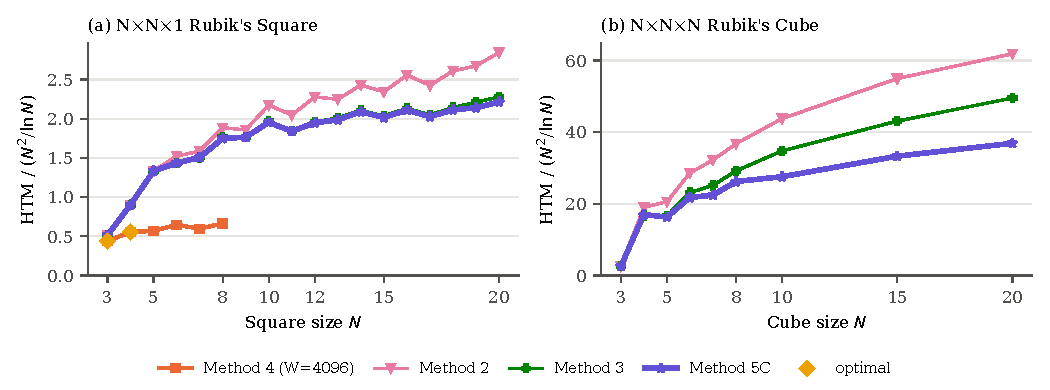
\includegraphics[width=\textwidth]{figures/scaling.pdf}
\caption{Solution length divided by $N^2/\ln N$, the growth rate of the worst case, for the Square (a) and the cube (b), random
states. A flat line would mean growth at the rate of the worst case. Means over solved states.}
\label{fig:scaling}
\end{figure*}

%% ---------------------------------------------------------------------
\subsection{Our methods against published numbers (Santa 2023)}
\label{sec:exp-published}

\begin{table*}[t]
\caption{Santa 2023 cube puzzles (standard one-colour-per-face goal, no wildcards), mean QTM, the competition's score. $n$: puzzles
per size; bound: counting lower bound (\S\ref{sec:bound}); B1--B3: external baselines (\S\ref{sec:baselines}); a superscript gives the
number of puzzles run when below $n$; ``--'' = not run. Last column: B1 / bound. \Mseven is in Table~\ref{tab:m7}.}
\label{tab:santa}
\small
\resizebox{\textwidth}{!}{%
\begin{tabular}{@{}rrr|rrr|rrrr|r@{}}
\toprule
$N$ & $n$ & bound & B1 KMCoders published & B2 KMCoders program, one run & B3 dwalton76 & \Msix & \FiveC & \Mthree & \Mtwo & B1 / bound \\
\midrule
4 & 43 & 37 & \textbf{64.1} & 66.7 & 77.0 & 88.6 & 109.4 & 217.5 & 229.3 & 266.9 & 1.81 \\
5 & 19 & 54 & \textbf{95.0} & 97.1 & 114.2 & 160.2 & 159.3 & 282.5 & 296.3 & 361.1 & 1.80 \\
6 & 6 & 80 & \textbf{158.3} & 161.0 & 179.3 & 324.0 & 276.0 & 503.0 & 534.7 & 696.3 & 2.00 \\
7 & 4 & 105 & \textbf{205.2} & 208.8 & 232.8 & 539.0 & 356.2 & 593.8 & 680.8 & 880.2 & 1.99 \\
8 & 3 & 138 & 294.7 & \textbf{291.3} & 310.7 & 923.3 & 468.7 & 856.0 & 993.3 & 1,297.3 & 2.12 \\
9 & 3 & 169 & 361.3 & \textbf{354.7} & 390.0 & 1,311.3 & 572.7 & 1,020.0 & 1,188.0 & 1,594.0 & 2.10 \\
10 & 4 & 208 & -- & \textbf{461.5} & 485.5 & 1,935.5 & 743.0 & 1,314.5 & 1,597.0 & 2,107.5 & 2.22 \\
\bottomrule

\end{tabular}}
\end{table*}

\paragraph{All methods on Santa 2023.}
Table~\ref{tab:santa} runs every cube method we have on the Santa puzzles, in the competition's metric. Our cluster methods, built
for the random benchmark and the half-turn metric, are far behind the competition solutions: \FiveC is \FiveCOverPubMin{}--\FiveCOverPubMax{}$\times$ B1, \Mthree
and \Mtwo more. dwalton76 is closer at $N=4$ but grows faster. \Msix, our reproduction of the KMCoders pipeline, is the best of these
from $N=6$ on. Only KMCoders' own program comes close to their published numbers, which is why \Mseven builds on it.

\begin{table}[t]
\caption{\Mseven against KMCoders' published solutions (B1), QTM per puzzle. \Cu{4}: best of 48 copies (beam variant, short
stage 2) and of 8 copies (default program); \Cu{5}: 24 copies with Kociemba's and with \texttt{nxopt}'s central \Cu{3}. ``best'':
\Mseven's answer (bold when shorter than B1). Last column: one run of their program (B2).}
\label{tab:m7}
\small\setlength{\tabcolsep}{3pt}
\begin{tabular}{@{}lrrrrrrr@{}}
\toprule
 & puzzle & B1 & 48 / 24 copies & 8 copies & \texttt{nxopt} & best & B2 \\
\midrule
\Cu{4} & 0150 & 66 & 66 & 66 & -- & 66 & 76 \\
\Cu{4} & 0151 & 68 & 60 & 70 & -- & \textbf{60} & 90 \\
\Cu{4} & 0152 & 56 & 60 & 72 & -- & 60 & 84 \\
\Cu{4} & 0153 & 65 & 67 & 69 & -- & 67 & 73 \\
\Cu{4} & 0154 & 71 & 65 & 71 & -- & \textbf{65} & 75 \\
\Cu{4} & 0155 & 64 & 66 & 64 & -- & 64 & 76 \\
\Cu{4} & 0157 & 65 & 63 & 73 & -- & \textbf{63} & 85 \\
\Cu{4} & 0158 & 63 & 63 & 65 & -- & 63 & 65 \\
\Cu{4} & 0159 & 57 & 63 & 57 & -- & 57 & 75 \\
\Cu{4} & 0161 & 60 & 62 & 72 & -- & 62 & 72 \\
\Cu{5} & 0210 & 99 & 101 & -- & 93 & \textbf{93} & 125 \\
\Cu{5} & 0212 & 99 & 103 & -- & 95 & \textbf{95} & 119 \\
\Cu{5} & 0213 & 104 & 102 & -- & 98 & \textbf{98} & 108 \\
\bottomrule

\end{tabular}
\end{table}

\paragraph{\Mseven reaches the published numbers.}
On the \MsevenNFour{} \Cu{4} puzzles, \Mseven's mean is \MsevenBestFour{} quarter turns against \MsevenPubFour{} for B1 and
\MsevenOneFour{} for one run of their program (B2): \MsevenWinsFour{} puzzles shorter than the published solution, \MsevenTiesFour{}
equal, \MsevenLossesFour{} longer (Table~\ref{tab:m7}). The 48-copy portfolio alone already averages \MsevenFortyEightMeanFour{},
equal to B1, at \MsevenCpuMinFour{} CPU-minutes per puzzle. Figure~\ref{fig:m7copies} shows why it works: the 48 copies of one puzzle
spread over \MsevenSpreadMinFour{}--\MsevenSpreadMaxFour{} quarter turns (all copies: \MsevenCopyMinFour{} to \MsevenCopyMaxFour{}, mean \MsevenCopyMeanFour{}), and the
published solution sits in the lower tail of that spread. Figure~\ref{fig:m7portfolio} shows the best of $k$ random copies: the mean
falls quickly at first and is still falling at $k=48$, so more copies (or seeds) should help further. On the \Cu{5}, with
Kociemba's central \Cu{3}, the 24-copy portfolio averages \MsevenKociembaFive{} against \MsevenPubFive{}; with \texttt{nxopt}'s optimal
stage it averages \MsevenNxoptMean{} against \MsevenNxoptPubMean{}: shorter than the published solution on all
\MsevenNxoptDone{} puzzles, by 4--6 quarter turns each, at \MsevenCpuMinFive{} CPU-minutes per puzzle. The optimal central stage
alone saves about 10 quarter turns per copy (34 to 24 on puzzle 210), more than the portfolio's gap to B1 at $N=4$.

\begin{figure}[t]
\centering
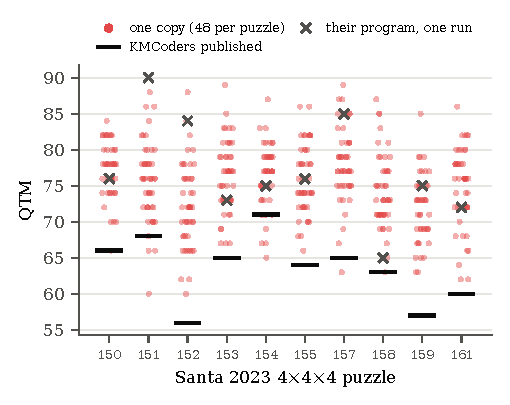
\includegraphics[width=\columnwidth]{figures/m7_copies.pdf}
\caption{\Mseven on the first 10 Santa \Cu{4} puzzles: QTM of each of the 48 symmetric copies (dots), KMCoders' published
solution (bar) and one run of their program on the unrotated puzzle (cross).}
\label{fig:m7copies}
\end{figure}

\begin{figure}[t]
\centering
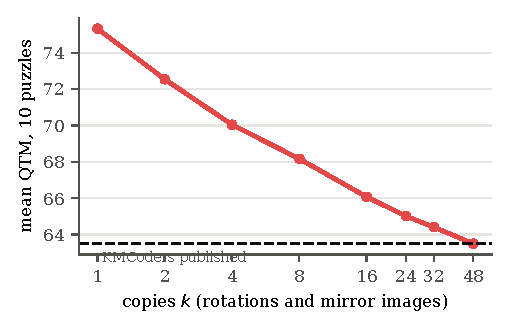
\includegraphics[width=\columnwidth]{figures/m7_portfolio.pdf}
\caption{Best of $k$ symmetric copies, averaged over the 10 \Cu{4} puzzles (and 200 random draws of the $k$ copies), against
KMCoders' published mean (dashed).}
\label{fig:m7portfolio}
\end{figure}

\paragraph{Time.}
Table~\ref{tab:santatime} gives the mean wall time per Santa puzzle. One run of KMCoders' program takes about a minute at $N=4$
and 22 minutes at $N=9$ on our shared machine, so \Mseven's $k$ copies cost $k$ times that; our cluster methods take seconds to
minutes even at $N=19$.

\begin{table}[t]
\caption{Mean wall time per Santa puzzle (seconds; shared 4-core machine, so indicative).}
\label{tab:santatime}
\small\setlength{\tabcolsep}{4pt}
\begin{tabular}{@{}rrrrrrr@{}}
\toprule
$N$ & B2 one run & B3 & \Msix & \FiveC & \Mthree & \Mtwo \\
\midrule
4 & 64 & 8 & 6 & 0 & 0 & 0 \\
5 & 131 & 22 & 10 & 1 & 0 & 0 \\
6 & 250 & 35 & 16 & 3 & 0 & 1 \\
7 & 473 & 38 & 23 & 6 & 0 & 2 \\
8 & 824 & -- & 36 & 11 & 1 & 4 \\
9 & 1,308 & -- & 46 & 17 & 1 & 4 \\
10 & -- & -- & 67 & 26 & 2 & 4 \\
\bottomrule

\end{tabular}
\end{table}

%% ---------------------------------------------------------------------
\subsection{How far from optimal?}
\label{sec:exp-bound}

Figure~\ref{fig:santaratio} divides each method's mean Santa length by the counting bound of \S\ref{sec:bound}. KMCoders' published
solutions are \PubOverBoundFour{}$\times$ the bound at $N=4$, \PubOverBoundTen{}$\times$ at $N=10$, \PubOverBoundNineteen{}$\times$ at
$N=19$ and \PubOverBoundThirtyThree{}$\times$ at $N=33$. On the Square, where we know the truth, the worst case is 1.5--1.7$\times$ the
bound (Table~\ref{tab:cal}), and typical optimal distances are lower still, so at small $N$ the published solutions are within a small
factor of optimal, and the room left grows with $N$. The growth has a clear cause: the published lengths are a near-constant
\PubPerNsqTen{}, \PubPerNsqNineteen{} and \PubPerNsqThirtyThree{}$\cdot N^2$ at $N=10$, 19 and 33, while the bound grows like
$N^2/\log N$. KMCoders' final stage fixes $O(1)$ pieces per 3-cycle, so it is $\Theta(N^2)$, although their stage 3 already contains
Demaine-style bulk commutators. A method that kept the parallelism of bulk commutators into the endgame, as \FiveC does on the random
benchmark, is the natural way to close this gap at large $N$; on Santa today, \FiveC's constant is still too large.

\begin{figure}[t]
\centering
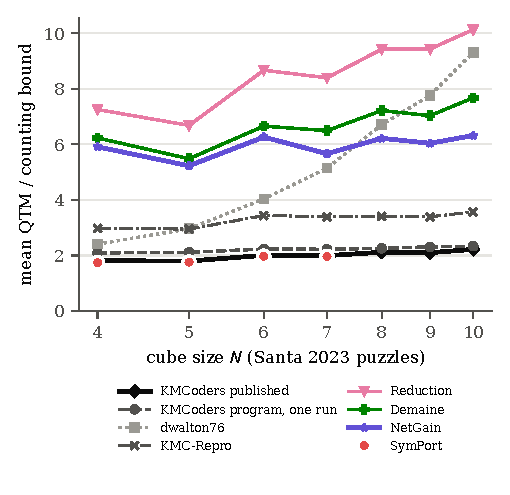
\includegraphics[width=\columnwidth]{figures/santa_ratio.pdf}
\caption{Mean Santa 2023 length divided by the counting lower bound, against $N$ (log scale). Methods shown only where they ran on
every puzzle of that size; \Mseven on the subsets of Table~\ref{tab:m7}.}
\label{fig:santaratio}
\end{figure}
